%\VignetteEngine{knitr::knitr}
% !Rnw weave = knitr
%\VignetteIndexEntry{MESgenCov: An R Package for ...}

\documentclass[11pt]{article}\usepackage[]{graphicx}\usepackage[]{color}
%% maxwidth is the original width if it is less than linewidth
%% otherwise use linewidth (to make sure the graphics do not exceed the margin)
\makeatletter
\def\maxwidth{ %
  \ifdim\Gin@nat@width>\linewidth
    \linewidth
  \else
    \Gin@nat@width
  \fi
}
\makeatother

\definecolor{fgcolor}{rgb}{0.345, 0.345, 0.345}
\newcommand{\hlnum}[1]{\textcolor[rgb]{0.686,0.059,0.569}{#1}}%
\newcommand{\hlstr}[1]{\textcolor[rgb]{0.192,0.494,0.8}{#1}}%
\newcommand{\hlcom}[1]{\textcolor[rgb]{0.678,0.584,0.686}{\textit{#1}}}%
\newcommand{\hlopt}[1]{\textcolor[rgb]{0,0,0}{#1}}%
\newcommand{\hlstd}[1]{\textcolor[rgb]{0.345,0.345,0.345}{#1}}%
\newcommand{\hlkwa}[1]{\textcolor[rgb]{0.161,0.373,0.58}{\textbf{#1}}}%
\newcommand{\hlkwb}[1]{\textcolor[rgb]{0.69,0.353,0.396}{#1}}%
\newcommand{\hlkwc}[1]{\textcolor[rgb]{0.333,0.667,0.333}{#1}}%
\newcommand{\hlkwd}[1]{\textcolor[rgb]{0.737,0.353,0.396}{\textbf{#1}}}%
\let\hlipl\hlkwb

\usepackage{framed}
\makeatletter
\newenvironment{kframe}{%
 \def\at@end@of@kframe{}%
 \ifinner\ifhmode%
  \def\at@end@of@kframe{\end{minipage}}%
  \begin{minipage}{\columnwidth}%
 \fi\fi%
 \def\FrameCommand##1{\hskip\@totalleftmargin \hskip-\fboxsep
 \colorbox{shadecolor}{##1}\hskip-\fboxsep
     % There is no \\@totalrightmargin, so:
     \hskip-\linewidth \hskip-\@totalleftmargin \hskip\columnwidth}%
 \MakeFramed {\advance\hsize-\width
   \@totalleftmargin\z@ \linewidth\hsize
   \@setminipage}}%
 {\par\unskip\endMakeFramed%
 \at@end@of@kframe}
\makeatother

\definecolor{shadecolor}{rgb}{.97, .97, .97}
\definecolor{messagecolor}{rgb}{0, 0, 0}
\definecolor{warningcolor}{rgb}{1, 0, 1}
\definecolor{errorcolor}{rgb}{1, 0, 0}
\newenvironment{knitrout}{}{} % an empty environment to be redefined in TeX

\usepackage{alltt}
\usepackage[left=1.1cm, top=2.54cm, right=1.1cm, bottom=2.54cm]{geometry}
\usepackage[utf8]{inputenc}
\usepackage[T1]{fontenc}
\usepackage{amsmath,amssymb,array}
\usepackage{booktabs}
\usepackage{caption}
\usepackage{cite}
\usepackage{colortbl}
\usepackage{comment}
\usepackage{float}
\usepackage{hyperref}
\usepackage{longtable}
\usepackage{multirow}
\usepackage{pdflscape}
\usepackage{subcaption}
\usepackage[table]{xcolor}
\usepackage{tabu}
\usepackage{threeparttable}
\usepackage[normalem]{ulem}
\usepackage{wrapfig}

 \geometry{
 a4paper,
 total={170mm,210mm},
 left=20mm,
 top=20mm,
 }


\title{MESgenCov: An R Package for generating covariance matrices \\ from precipitation chemistry data}
\author{Hessa Al-Thani$^1$ \qquad Jon Lee$^2$\\[0.35cm]
  {\small Dept. of Industrial and Operations Engineering, Univ. of Michigan, Ann Arbor, MI 48105 USA }\\[0.35cm]{\small{$^1$hessakh@umich.edu}} \qquad {\small{$^2$jonxlee@umich.edu}}
}
\date{\textbf{MESgenCov} 0.1.0  }
%
\IfFileExists{upquote.sty}{\usepackage{upquote}}{}
\begin{document}



\maketitle

\begin{abstract}
  We present an R package for temporally fitting multivariate precipitation chemistry data and extracting a covariance matrix
for use in MES (maximum-entropy sampling).
 We provide multiple functionalities for modeling and model assessment. The package uses data from the NADP/NTN (National Atmospheric Deposition Program / National Trends Network) on their set of more than 370 monitoring sites, 1978--present. The user specifies the sites, chemicals and time period desired, fits a user-defined univariate model for each site and chemical selected, and produces a covariance matrix for use by MES algorithms.

\end{abstract}

\section{The MES problem}

The MES (maximum-entropy sampling) problem (see \cite{ShewryWynn,SebWynn,FedorovLee,LeeEnv}) has been applied to many domains where the objective is to determine a most informative subset $S$, of presepcified size $s$, from a set of $n$ Gaussian variables $N$. This is done by seeking to maximize the (log) determinant of the covariance matrix for some $S \subseteq N$ with $|S|=s$ (see \cite{KLQ,LeeConstrained,AFLW_Using,LeeWilliams_ILP,HLW,AnstreicherLee_Masked,BurerLee,AnstreicherBQPEntropy,linx}). A key area of application has been in environmental montoring (see \cite{Zidek1,Zidek2,Zidek3}, for example).
In this R package, we use  precipitation chemistry data
(ammonium,
calcium,
chloride,
hydrogen,
 magnesium,
 nitrate,
pH,
 potassium,
  sodium, and
sulfate) gathered by the NADP (National Atmospheric Deposition Program) at over 370 sites across the U.S.A. (see \cite{NADPNTN}).
For these instances of the MES problem, $n$ \emph{user-specified} site/chemical pairs comprise $N$.
%%add a bit on generalized getCov after finishing the function

\section{NADP data description}

The NADP maintains the NTN (National Trends Network); this network measures the chemistry of precipitation at monitoring sites across the
U.S.A. Our R package makes use of the weekly data measuring  mg/L of chemicals, such as sulfates, in collected precipitation. We also use the daily data measuring precipitation at each site. Both datasets are available in our package and can be loaded respectively as


\begin{knitrout}
\definecolor{shadecolor}{rgb}{0.969, 0.969, 0.969}\color{fgcolor}\begin{kframe}
\begin{alltt}
 \hlkwd{data}\hlstd{(}\hlstr{"weeklyConc"}\hlstd{)}
 \hlkwd{data}\hlstd{(}\hlstr{"preDaily"}\hlstd{)}
\end{alltt}
\end{kframe}
\end{knitrout}

A full description of the data can be obtained at \href{http://NADP.slh.wisc.edu/data/ntn/meta/ntn-weekly-Meta.pdf}{NADP/NTN weekly meta}. For a full description of the daily precipitation data, see \href{http://NADP.slh.wisc.edu/data/ntn/meta/ntn-daily-Meta.pdf}{NADP/NTN daily meta}. Small snapshots of the data can also be viewed using:

\begin{knitrout}
\definecolor{shadecolor}{rgb}{0.969, 0.969, 0.969}\color{fgcolor}\begin{kframe}
\begin{alltt}
  \hlstd{weeklyConc[}\hlnum{1}\hlopt{:}\hlnum{5}\hlstd{,}\hlnum{1}\hlopt{:}\hlnum{5}\hlstd{]}
\end{alltt}
\begin{verbatim}
##   siteID              dateon             dateoff yrmonth    ph
## 1   AB32 2016-09-13 18:40:00 2016-09-20 15:10:00  201609 -9.00
## 2   AB32 2016-09-20 15:15:00 2016-09-28 16:00:00  201609 -9.00
## 3   AB32 2016-09-28 16:00:00 2016-10-05 16:55:00  201610  6.56
## 4   AB32 2016-10-05 16:55:00 2016-10-11 17:00:00  201610 -9.00
## 5   AB32 2016-10-11 17:00:00 2016-10-18 20:00:00  201610 -9.00
\end{verbatim}
\end{kframe}
\end{knitrout}

This outputs the first 6 rows, first 4 columns and 9th column of the weekly raw data, columns 5 to 8 contain data that isn't relevant to our analysis.
\section{MESgenCov implementation}

 The \textbf{MESgenCov} package contains functions in the \texttt{S3} class to create a covariance matrix from the desired subset of NADP data. The function \verb;getCov(); returns a covariance matrix, a list of univariate model summaries, and a table of normality tests produced by the MVN R package. The covariance matrix is produced from a subset of the NADP/NTN data that is specified by the user. For sites with missing data, \verb;getCov(); will fill in predicted values based on the univariate model for each site (see section \ref{sec:3.1}). To avoid sites with a small sample size for the specified time-frame, the function \verb;getSites(); outputs a vector of the sites with the largest sample of data for a given time-frame and measured chemical (see section \ref{sec:3.2}). To find sites that are spatially ``spread out'' but have at least some specified sample size, the function \verb;maxDistSites(); can be used (see section \ref{sec:3.2}).

  \subsection{getCov}
  \label{sec:3.1}
  \subsubsection{Input}

  \verb;getCov(); takes a 15 column data frame as input where each column corresponds to one of the following user-specifications, given in the table below.The 15 specifications in the input allow the user to specify the subset of data to analyze and gives the user options in displaying different parts of the analysis.

  %%table



\begin{knitrout}
\definecolor{shadecolor}{rgb}{0.969, 0.969, 0.969}\color{fgcolor}\begin{table}[H]
\centering\begin{table}[H]
\centering
\begin{tabular}{>{\bfseries\leavevmode\color{black}}l>{\raggedright\arraybackslash}p{30em}}
\toprule
Arguments & Definition\\
\midrule
\rowcolor{gray!6}  weeklyB & TRUE if weekly data should be analyzed and FALSE if monthly data should be analyzed\\
startdateStr & Date and time of when to start analyzing the data, in the format = “m/d/y H:M”\\
\rowcolor{gray!6}  enddateStr & Date and time of when to stop analyzing the data, in the format = “m/d/y H:M”\\
comp & Vector of strings of pollutants or acidity levels to be analyzed, the pollutants name should be used as it appears in weeklyCSV\\
\rowcolor{gray!6}  use36 & TRUE if default 36 sites should be added, FALSE otherwise\\
\addlinespace
siteAdd & List of strings of siteIDs that should be analyzed\\
\rowcolor{gray!6}  outlierDatesbySite & List of sites where outliers should be analyzed\\
siteOutliers & List of sites where outliers should be removed\\
\rowcolor{gray!6}  removeOutliers & Specify siteID string for outlier analysis\\
plotMulti & TRUE if multivariate analysis plots should be displayed, FALSE otherwise\\
\addlinespace
\rowcolor{gray!6}  sitePlot & Specify siteID to be plotted\\
plotAll & TRUE if plots for all sites should be displayed, FALSE otherwise\\
\rowcolor{gray!6}  writeMat & TRUE if  .mat file of the resulting covariance matrix should be written in the working directory\\
seas & Approximate periodicity of data, typically 12 for monthly data and 52 for weekly data\\
\rowcolor{gray!6}  r & Integer <=5, see univariate model\\
k & Integer <= 5, see univariate model\\
\bottomrule
\end{tabular}
\end{table}
\end{table}


\end{knitrout}
A default set of inputs can be found in the internally stored dataframe "defaultInput". After storing it in a variable in the user's workspace the input can be changed in the following way:
\begin{knitrout}
\definecolor{shadecolor}{rgb}{0.969, 0.969, 0.969}\color{fgcolor}\begin{kframe}
\begin{alltt}
 \hlkwd{data}\hlstd{(}\hlstr{"defaultInput"}\hlstd{)}
 \hlstd{df} \hlkwb{<-} \hlstd{defaultInput}
 \hlstd{df}
\end{alltt}
\begin{verbatim}
##   weeklyB   startdateStr     enddateStr comp use36 siteAdd
## 1   FALSE 01/01/83 00:00 12/31/86 00:00  SO4  TRUE    NULL
##   outlierDatesbySite siteOutliers removeOutliers plotMulti sitePlot
## 1               NULL         NULL           NULL     FALSE     NULL
##   plotAll writeMat seas r k
## 1   FALSE    FALSE   12 1 1
\end{verbatim}
\begin{alltt}
 \hlstd{df}\hlopt{$}\hlstd{enddateStr}   \hlkwb{<-} \hlstr{"12/31/88 00:00"}
\end{alltt}
\end{kframe}
\end{knitrout}

\subsubsection{Output}


The function \texttt{getCov} produces the following outputs:
%


\begin{knitrout}
\definecolor{shadecolor}{rgb}{0.969, 0.969, 0.969}\color{fgcolor}\begin{table}[H]
\centering\begin{table}[H]
\centering
\begin{tabular}{>{\bfseries\leavevmode\color{black}}l>{\raggedright\arraybackslash}p{30em}}
\toprule
Output & Definition\\
\midrule
\rowcolor{gray!6}  cov & Covariance matrix produced by univariate model residuals\\
listMod & List of univariate model summaries produced by lm()\\
\rowcolor{gray!6}  sites & List of sites that were analyzed\\
mvn & Output of the MVN package\\
\rowcolor{gray!6}  univariateTest & univariate test output, also by the MVN package\\
\addlinespace
residualData & Data frame of residuals produced by the univariate model\\
\rowcolor{gray!6}  residualDataNA & Data frame of residuals, where missing values are ledt as NA\\
rosnerTest & Output of the rosner test for outlier analysis produced by the EnvStats package\\
\rowcolor{gray!6}  pred & List of predicted values produced by the univariate model for each site\\
noutliers & Number of outliers detected by the outlier analysis, default is 0 if no sites are analyzed for outliers\\
\bottomrule
\end{tabular}
\end{table}
\end{table}


\end{knitrout}

Here we present some examples of the various outputs.

\begin{enumerate}

\item Multivariate and univariate normality
\begin{knitrout}
\definecolor{shadecolor}{rgb}{0.969, 0.969, 0.969}\color{fgcolor}\begin{kframe}
\begin{alltt}
  \hlstd{df}\hlopt{$}\hlstd{plotMulti}    \hlkwb{<-} \hlnum{TRUE}
  \hlstd{df}\hlopt{$}\hlstd{k}            \hlkwb{<-} \hlnum{3}
  \hlstd{g} \hlkwb{<-}\hlkwd{getCov}\hlstd{(df)}
\end{alltt}
\end{kframe}
\end{knitrout}

\begin{center}
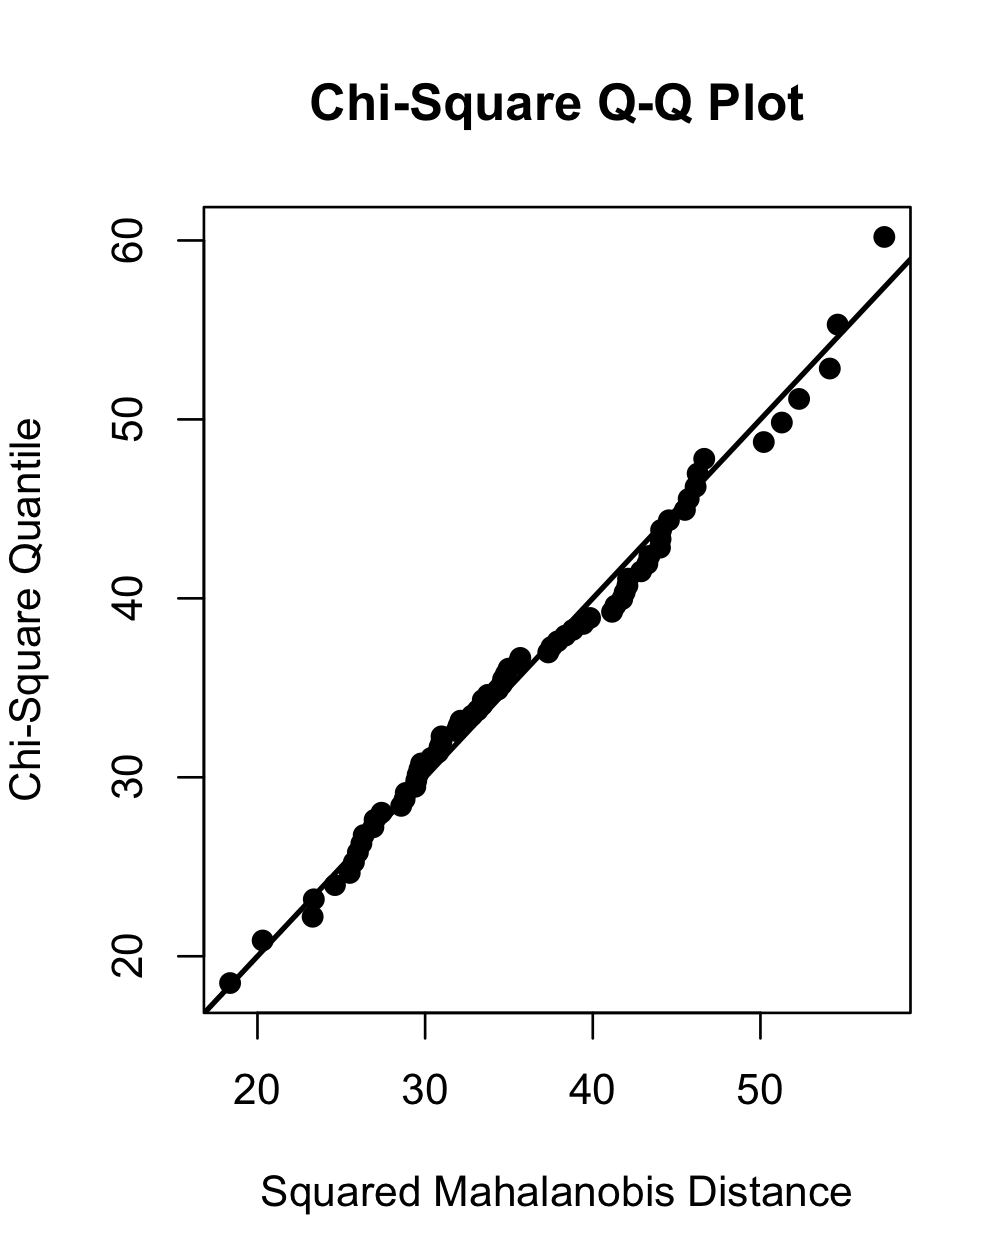
\includegraphics[width = 75mm]{pic1GetCov}
\end{center}



\begin{knitrout}
\definecolor{shadecolor}{rgb}{0.969, 0.969, 0.969}\color{fgcolor}\begin{kframe}
\begin{alltt}
  \hlstd{g}\hlopt{$}\hlstd{univariateTest[}\hlnum{1}\hlopt{:}\hlnum{5}\hlstd{,]}
\end{alltt}
\begin{verbatim}
##           Test  Variable Statistic   p value Normality
## 1 Shapiro-Wilk  AL10SO4     0.9347   0.001      NO    
## 2 Shapiro-Wilk  IL11SO4     0.9894  0.8121      YES   
## 3 Shapiro-Wilk  IL18SO4     0.9909  0.8854      YES   
## 4 Shapiro-Wilk  IL19SO4     0.9183   2e-04      NO    
## 5 Shapiro-Wilk  IL35SO4     0.8709  <0.001      NO
\end{verbatim}
\end{kframe}
\end{knitrout}
%%



\item Outlier test for specific tests
\begin{knitrout}
\definecolor{shadecolor}{rgb}{0.969, 0.969, 0.969}\color{fgcolor}\begin{kframe}
\begin{alltt}
  \hlstd{df}\hlopt{$}\hlstd{siteOutliers} \hlkwb{<-} \hlkwd{list}\hlstd{(}\hlkwd{c}\hlstd{(}\hlstr{"IN41"}\hlstd{))}
  \hlstd{df}\hlopt{$}\hlstd{sitePlot}     \hlkwb{<-} \hlstr{"IN41"}
  \hlstd{g} \hlkwb{<-} \hlkwd{getCov}\hlstd{(df)}
  \hlstd{i} \hlkwb{<-} \hlkwd{match}\hlstd{(}\hlstr{"IN41"}\hlstd{,g}\hlopt{$}\hlstd{sites)}
  \hlstd{g}\hlopt{$}\hlstd{rosnerTest[[i]]}\hlopt{$}\hlstd{all.stats}
\end{alltt}
\begin{verbatim}
##   i       Mean.i      SD.i      Value Obs.Num    R.i+1 lambda.i+1 Outlier
## 1 0 -0.006929523 0.2813805 -0.9358517      25 3.301302   3.267957    TRUE
## 2 1  0.006153889 0.2603946 -0.7193545      30 2.786188   3.262821   FALSE
## 3 2  0.016518294 0.2470843  0.7215347      66 2.853344   3.257596   FALSE
\end{verbatim}
\end{kframe}
\end{knitrout}

\begin{knitrout}
\definecolor{shadecolor}{rgb}{0.969, 0.969, 0.969}\color{fgcolor}\begin{kframe}
\begin{alltt}
  \hlstd{df}\hlopt{$}\hlstd{outlierDatesbySite} \hlkwb{<-} \hlkwd{c}\hlstd{(}\hlstr{"IN41"}\hlstd{,}\hlnum{25}\hlstd{)}
  \hlkwd{getCov}\hlstd{(df)}
\end{alltt}
\end{kframe}
\end{knitrout}
\begin{center}
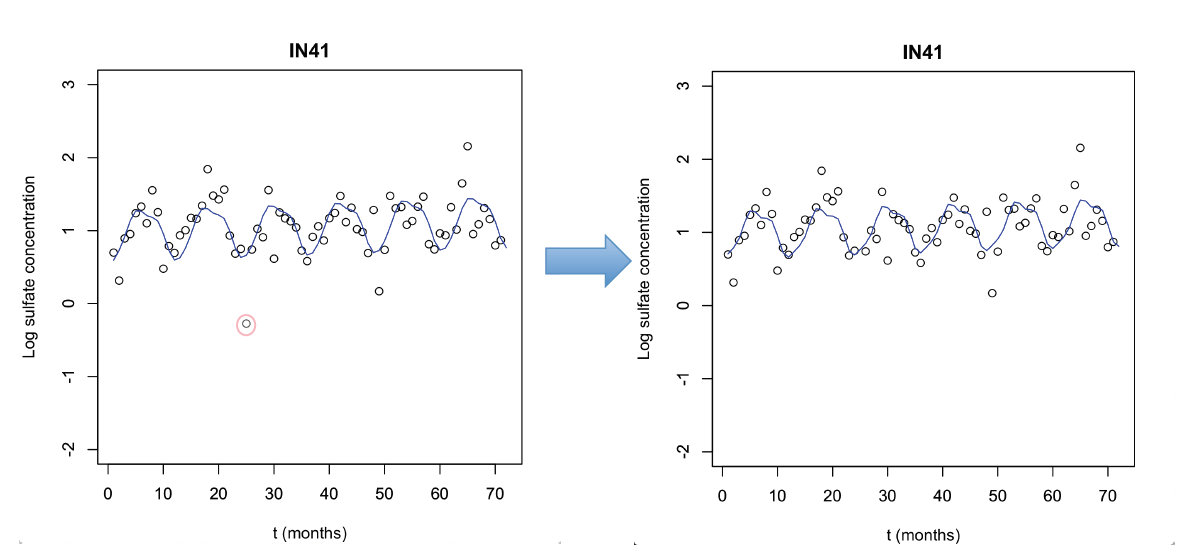
\includegraphics[width = 75mm]{IN41trans}
\end{center}
%%
For all sites,

\begin{knitrout}
\definecolor{shadecolor}{rgb}{0.969, 0.969, 0.969}\color{fgcolor}\begin{kframe}
\begin{alltt}
  \hlstd{df}\hlopt{$}\hlstd{siteOutliers}   \hlkwb{<-} \hlkwd{list}\hlstd{(g}\hlopt{$}\hlstd{sites)}
  \hlstd{df}\hlopt{$}\hlstd{removeOutliers} \hlkwb{<-} \hlkwd{list}\hlstd{(g}\hlopt{$}\hlstd{sites)}
  \hlstd{g} \hlkwb{<-} \hlkwd{getCov}\hlstd{(df)}
\end{alltt}
\end{kframe}
\end{knitrout}



\item Plot all sites
\begin{knitrout}
\definecolor{shadecolor}{rgb}{0.969, 0.969, 0.969}\color{fgcolor}\begin{kframe}
\begin{alltt}
  \hlstd{df}\hlopt{$}\hlstd{plotAll} \hlkwb{<-} \hlnum{TRUE}
  \hlkwd{getCov}\hlstd{(df)}
\end{alltt}
\end{kframe}
\end{knitrout}

\begin{center}
  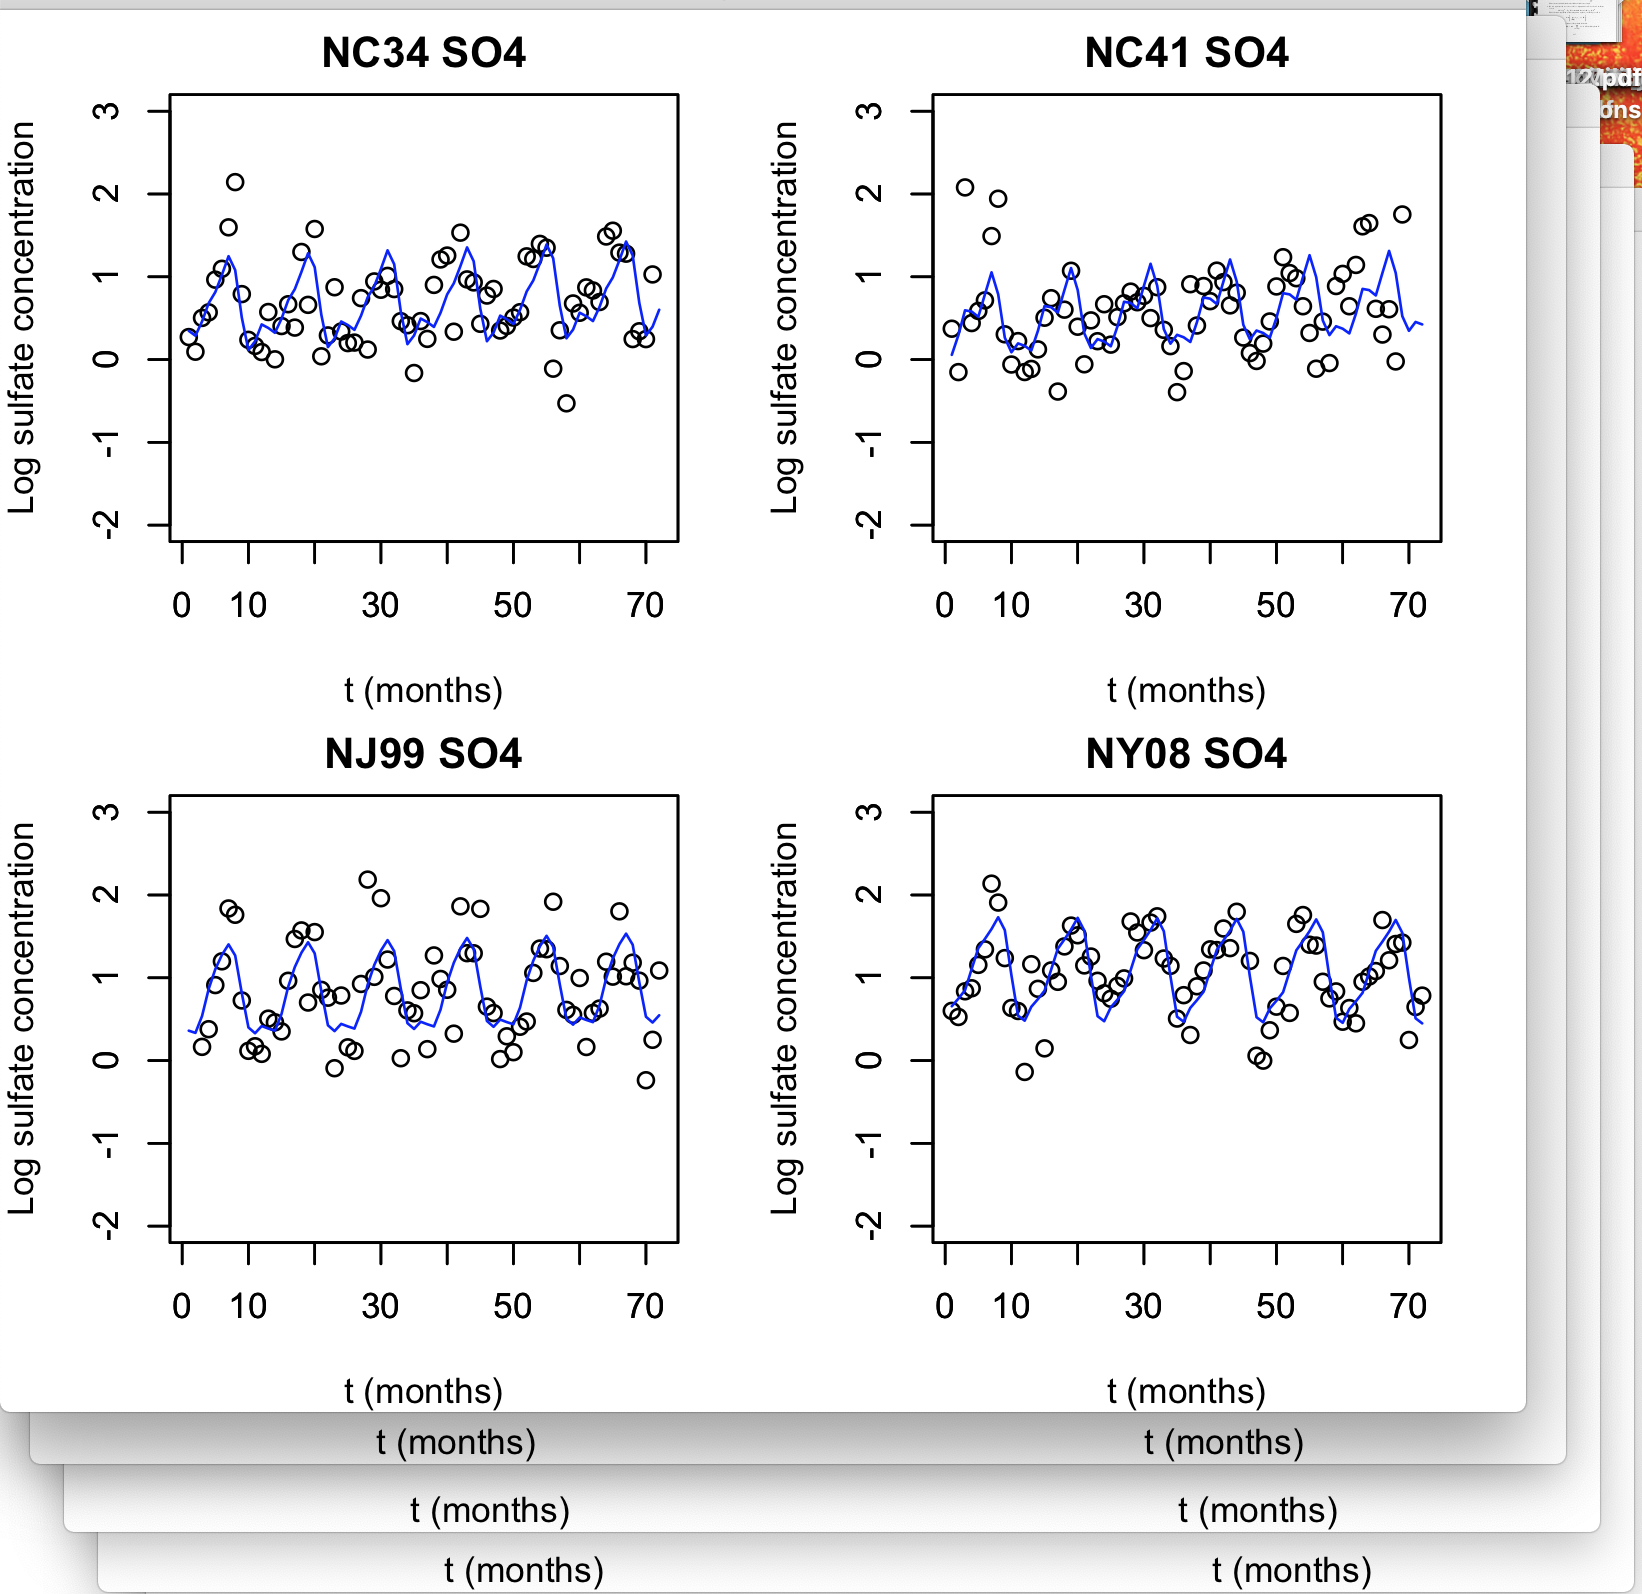
\includegraphics[width=75mm]{plotAll}
\end{center}

\item Covariance matrix
%%%%Parsing results
\begin{knitrout}
\definecolor{shadecolor}{rgb}{0.969, 0.969, 0.969}\color{fgcolor}\begin{kframe}
\begin{alltt}
  \hlstd{df}\hlopt{$}\hlstd{use36}              \hlkwb{<-} \hlnum{FALSE}
  \hlstd{df}\hlopt{$}\hlstd{siteAdd}            \hlkwb{<-} \hlkwd{list}\hlstd{(}\hlkwd{c}\hlstd{(}\hlstr{"OH71"}\hlstd{,} \hlstr{"WV18"}\hlstd{,} \hlstr{"MI53"}\hlstd{))}
  \hlstd{df}\hlopt{$}\hlstd{sitePlot}           \hlkwb{<-} \hlkwa{NULL}
  \hlstd{df}\hlopt{$}\hlstd{siteOutliers}       \hlkwb{<-} \hlkwa{NULL}
  \hlstd{df}\hlopt{$}\hlstd{outlierDatesbySite} \hlkwb{<-} \hlkwa{NULL}
  \hlstd{df}\hlopt{$}\hlstd{removeOutliers}     \hlkwb{<-} \hlkwa{NULL}
  \hlstd{g}                     \hlkwb{<-} \hlkwd{getCov}\hlstd{(df)}
  \hlkwd{round}\hlstd{(g}\hlopt{$}\hlstd{cov,}\hlkwc{digits} \hlstd{=} \hlnum{4}\hlstd{)}
\end{alltt}
\begin{verbatim}
##         OH71SO4 WV18SO4 MI53SO4
## OH71SO4  0.0770  0.0231  0.0092
## WV18SO4  0.0231  0.0911  0.0124
## MI53SO4  0.0092  0.0124  0.1096
\end{verbatim}
\end{kframe}
\end{knitrout}

\item Save covariance matrix as .mat file

This is done by simply setting the 5th last input to TRUE then the .mat file will be saved to the user's current working directory.

\begin{knitrout}
\definecolor{shadecolor}{rgb}{0.969, 0.969, 0.969}\color{fgcolor}\begin{kframe}
\begin{alltt}
  \hlstd{df}\hlopt{$}\hlstd{writeMat} \hlkwb{<-} \hlnum{TRUE}
  \hlstd{g}           \hlkwb{<-} \hlkwd{getCov}\hlstd{(df)}
\end{alltt}
\end{kframe}
\end{knitrout}

In the case that the user has already generated an output by the function \texttt{getCov()}, it is possible to also create the mat file in the following way.


\begin{knitrout}
\definecolor{shadecolor}{rgb}{0.969, 0.969, 0.969}\color{fgcolor}\begin{kframe}
\begin{alltt}
  \hlkwd{library}\hlstd{(rmatio)}
  \hlkwd{write.mat}\hlstd{(g}\hlopt{$}\hlstd{cov,}\hlkwc{filename} \hlstd{=} \hlstr{"covariance1.mat"}\hlstd{)}
\end{alltt}
\end{kframe}
\end{knitrout}
\item Univariate model summaries
%%%%Parsing results
\begin{knitrout}
\definecolor{shadecolor}{rgb}{0.969, 0.969, 0.969}\color{fgcolor}\begin{kframe}
\begin{alltt}
  \hlstd{sites}  \hlkwb{<-} \hlstd{g}\hlopt{$}\hlstd{sites}
  \hlstd{i} \hlkwb{=} \hlkwd{match}\hlstd{(}\hlkwd{c}\hlstd{(}\hlstr{"OH71"}\hlstd{),sites)}
  \hlstd{g}\hlopt{$}\hlstd{listMod[i]}
\end{alltt}
\begin{verbatim}
## [[1]]
## 
## Call:
## lm(formula = y1 ~ I(cos(t * (2 * pi/seas))^p) + I(sin(t * (2 * 
##     pi/seas))^p) + I(cos(t * (2 * pi/seas) * 2)^p) + I(sin(t * 
##     (2 * pi/seas) * 2)^p) + I(cos(t * (2 * pi/seas) * 3)^p) + 
##     I(sin(t * (2 * pi/seas) * 3)^p) + I(t), data = df)
## 
## Residuals:
##      Min       1Q   Median       3Q      Max 
## -0.52359 -0.16772 -0.01885  0.18184  0.90868 
## 
## Coefficients:
##                                   Estimate Std. Error t value Pr(>|t|)    
## (Intercept)                      1.1110107  0.0702653  15.812  < 2e-16 ***
## I(cos(t * (2 * pi/seas))^p)     -0.3541145  0.0487427  -7.265 6.37e-10 ***
## I(sin(t * (2 * pi/seas))^p)     -0.1108821  0.0491147  -2.258   0.0274 *  
## I(cos(t * (2 * pi/seas) * 2)^p)  0.0499868  0.0487427   1.026   0.3090    
## I(sin(t * (2 * pi/seas) * 2)^p)  0.0796743  0.0488005   1.633   0.1075    
## I(cos(t * (2 * pi/seas) * 3)^p)  0.0390617  0.0487427   0.801   0.4259    
## I(sin(t * (2 * pi/seas) * 3)^p)  0.0535530  0.0487427   1.099   0.2760    
## I(t)                             0.0009172  0.0016779   0.547   0.5865    
## ---
## Signif. codes:  0 '***' 0.001 '**' 0.01 '*' 0.05 '.' 0.1 ' ' 1
## 
## Residual standard error: 0.2923 on 64 degrees of freedom
## Multiple R-squared:  0.4995,	Adjusted R-squared:  0.4448 
## F-statistic: 9.125 on 7 and 64 DF,  p-value: 9.097e-08
\end{verbatim}
\end{kframe}
\end{knitrout}

\item Output all MVN package analysis\\
\noindent
\\
\noindent
The following output is a call to the MVN package that produces mutivariate analysis based on the Mardia method, univariate analysis based on the Shapiro-Wilson method and an multivariate outlier test that is presented as a plot and not as an output in the user's R console.


\begin{knitrout}
\definecolor{shadecolor}{rgb}{0.969, 0.969, 0.969}\color{fgcolor}\begin{kframe}
\begin{alltt}
  \hlstd{g}\hlopt{$}\hlstd{mvn}
\end{alltt}
\begin{verbatim}
## $multivariateNormality
##              Test        Statistic             p value Result
## 1 Mardia Skewness  24.362552007168  0.0066940769960186     NO
## 2 Mardia Kurtosis 2.59883767062138 0.00935399956866512     NO
## 3             MVN             <NA>                <NA>     NO
## 
## $univariateNormality
##           Test  Variable Statistic   p value Normality
## 1 Shapiro-Wilk  OH71SO4     0.9593    0.0201    NO    
## 2 Shapiro-Wilk  WV18SO4     0.9823    0.4073    YES   
## 3 Shapiro-Wilk  MI53SO4     0.9487    0.0053    NO    
## 
## $Descriptives
##          n          Mean   Std.Dev       Median        Min       Max
## OH71SO4 72 -1.025964e-17 0.2775010 -0.018850157 -0.5235855 0.9086803
## WV18SO4 72 -6.613633e-18 0.3018523  0.003571524 -0.7192734 0.7195297
## MI53SO4 72 -1.356006e-18 0.3310569 -0.012777134 -0.5260723 1.2265622
##               25th      75th      Skew   Kurtosis
## OH71SO4 -0.1677203 0.1818372 0.6819771 1.10314285
## WV18SO4 -0.1868506 0.1776964 0.2203785 0.05048396
## MI53SO4 -0.2596244 0.2318249 0.7628797 0.88211091
## 
## $multivariateOutliers
##   Observation Mahalanobis Distance Outlier
## 1           1               16.524    TRUE
## 2           2               16.144    TRUE
## 3           3               15.684    TRUE
## 4           4               15.421    TRUE
## 5           5               10.627    TRUE
## 6           6               10.616    TRUE
## 7           7                9.477    TRUE
\end{verbatim}
\end{kframe}
\end{knitrout}

The specific call the the MVN package is,

\begin{knitrout}
\definecolor{shadecolor}{rgb}{0.969, 0.969, 0.969}\color{fgcolor}\begin{kframe}
\begin{alltt}
 \hlkwd{mvn}\hlstd{(dfRes[,}\hlopt{-}\hlnum{1}\hlstd{],} \hlkwc{subset} \hlstd{=} \hlkwa{NULL}\hlstd{,} \hlkwc{mvnTest} \hlstd{=} \hlstr{"mardia"}\hlstd{,} \hlkwc{covariance} \hlstd{=} \hlnum{TRUE}\hlstd{,}
     \hlkwc{tol} \hlstd{=} \hlnum{1e-25}\hlstd{,} \hlkwc{alpha} \hlstd{=} \hlnum{0.5}\hlstd{,} \hlkwc{scale} \hlstd{=} \hlnum{FALSE}\hlstd{,} \hlkwc{desc} \hlstd{=} \hlnum{TRUE}\hlstd{,} \hlkwc{transform} \hlstd{=} \hlstr{"none"}\hlstd{,}
     \hlkwc{univariateTest} \hlstd{=} \hlstr{"SW"}\hlstd{,}  \hlkwc{univariatePlot} \hlstd{=} \hlstr{"none"}\hlstd{,} \hlkwc{multivariatePlot} \hlstd{=}\hlstr{"none"}\hlstd{,}
     \hlkwc{multivariateOutlierMethod} \hlstd{=} \hlstr{"none"}\hlstd{,} \hlkwc{bc} \hlstd{=} \hlnum{FALSE}\hlstd{,} \hlkwc{bcType} \hlstd{=} \hlstr{"rounded"}\hlstd{,}
     \hlkwc{showOutliers} \hlstd{=} \hlnum{FALSE}\hlstd{,} \hlkwc{showNewData} \hlstd{=} \hlnum{FALSE}\hlstd{)}
\end{alltt}
\end{kframe}
\end{knitrout}

See \cite{MVN} for details on the MVN package.

\item Output dataframe of residuals\\
\begin{knitrout}
\definecolor{shadecolor}{rgb}{0.969, 0.969, 0.969}\color{fgcolor}\begin{kframe}
\begin{alltt}
  \hlstd{g}\hlopt{$}\hlstd{residualData[}\hlnum{1}\hlopt{:}\hlnum{5}\hlstd{,]}
\end{alltt}
\begin{verbatim}
##      OH71SO4     WV18SO4    MI53SO4
## 1 -0.1863739 -0.17114817  0.4782343
## 2 -0.2965845 -0.15398625  0.2875634
## 3 -0.4194283 -0.02188007 -0.5112095
## 4 -0.1446214 -0.49188947 -0.3921147
## 5 -0.5235855 -0.53657443  0.0579487
\end{verbatim}
\end{kframe}
\end{knitrout}


\end{enumerate}

  \subsection{Functions for getting a vector of sites}
    \label{sec:3.2}
 \texttt{getCov()} takes site lists as input, the function \texttt{getSites()} produces a list of sites with available data for a specified time frame. The code below produces a list of 36 sites with the most weekly data between the years 1983-1986.

\begin{knitrout}
\definecolor{shadecolor}{rgb}{0.969, 0.969, 0.969}\color{fgcolor}\begin{kframe}
\begin{alltt}
  \hlstd{result} \hlkwb{<-} \hlkwd{getSites}\hlstd{(}\hlstr{"01/01/83 00:00"}\hlstd{,} \hlstr{"12/31/86 00:00"}\hlstd{,}\hlnum{36}\hlstd{,}\hlnum{104}\hlstd{,}\hlstr{"SO4"}\hlstd{,}\hlstr{""}\hlstd{)}
  \hlstd{result}\hlopt{$}\hlstd{finalList}
\end{alltt}
\begin{verbatim}
##  [1] "OH71" "NY08" "WV18" "MI53" "NH02" "OH49" "PA42" "ME09" "IN34" "MA13"
## [11] "NY52" "NY10" "WA14" "NY20" "OH17" "ME00" "TN00" "IL63" "MI99" "WI28"
## [21] "IN41" "PA29" "WI36" "ME02" "MI09" "MO05" "NC03" "NJ99" "PA15" "CO19"
## [31] "MN18" "WI37" "AR27" "KS31" "ME98" "MO03"
\end{verbatim}
\end{kframe}
\end{knitrout}

The 4th input specifies the minimum sample of weekly data required to be included in the produced list and the last input tells the function to only look at sites in the North Eastern region of the US. Other options for region "W","S","N", see Appendix A for the precise geographic split.

\begin{knitrout}
\definecolor{shadecolor}{rgb}{0.969, 0.969, 0.969}\color{fgcolor}\begin{kframe}
\begin{alltt}
  \hlstd{NSites} \hlkwb{<-} \hlkwd{getSites}\hlstd{(}\hlstr{"01/01/83 00:00"}\hlstd{,} \hlstr{"12/31/86 00:00"}\hlstd{,}\hlnum{36}\hlstd{,}\hlnum{104}\hlstd{,}\hlstr{"SO4"}\hlstd{,}\hlstr{"N"}\hlstd{)}
  \hlstd{NSites}\hlopt{$}\hlstd{finalList}
\end{alltt}
\begin{verbatim}
##  [1] "OH71" "NY08" "MI53" "NH02" "OH49" "PA42" "ME09" "IN34" "MA13" "NY52"
## [11] "NY10" "NY20" "OH17" "ME00" "MI99" "WI28" "IN41" "PA29" "WI36" "ME02"
## [21] "MI09" "NJ99" "PA15" "MN18" "WI37" "ME98" "IL11" "IL18" "MN16" "MI26"
## [31] "NE15" "VT01" "NY99" "MA01" "MA08" "MN27"
\end{verbatim}
\end{kframe}
\end{knitrout}

The function \texttt{maxDistSites()} prioritizes sites that are farther away from each other.

\begin{knitrout}
\definecolor{shadecolor}{rgb}{0.969, 0.969, 0.969}\color{fgcolor}\begin{kframe}
\begin{alltt}
  \hlstd{maxdist} \hlkwb{<-} \hlkwd{maxDistSites}\hlstd{(}\hlstr{"01/01/83 00:00"}\hlstd{,} \hlstr{"12/31/86 00:00"}\hlstd{,}\hlnum{36}\hlstd{,}\hlnum{104}\hlstd{,}\hlstr{"SO4"}\hlstd{,}\hlnum{1}\hlstd{)}
  \hlstd{maxdist}\hlopt{$}\hlstd{finalList}
\end{alltt}
\begin{verbatim}
##  [1] "OH71" "WA14" "TX04" "FL11" "ME00" "WY06" "MN27" "LA12" "CA45" "OK00"
## [11] "NY99" "GA41" "MI99" "AZ03" "MT05" "NC35" "MO05" "CO00" "WY99" "IN34"
## [21] "KY03" "MI09" "FL03" "MA01" "OR10" "PA42" "AR27" "MN16" "TX21" "VT99"
## [31] "NE15" "VA13" "CO15" "CO22" "NY52" "AR02" "WI28"
\end{verbatim}
\end{kframe}
\end{knitrout}

  \subsection{Lambert's W transformation on univariate data}
    \label{sec:3.3}
  For a number of sites the resdiuals produced by the deterministic model have skewed distributions with heavy tails. In particular, this is the case for many sites when the sample of data is taken over a period longer than 4 years. To deal with this issue we've incorporated functions from the LambertW package (see \cite{LambertW})in the function \texttt{lambertWtransform()} that will allow a user to transform the residuals produced by the deterministic univariate model. The LambertW package estimates the parameters that fit a LamberW distribution on the given univariate data. Then the underlying gaussian distribution implied by the LambertW distribution is extracted and is used for the multivariate analysis in the function \texttt{lambertWtransform()}. The \texttt{lambertWtransform()} function takes the following as input: a dataframe of residuals, and two binary inputs specifying whether to plot the multivariate qq plot and whether to produce the mat file containing the covariance matrix with the Lambert W transformed residuals. Details on the algorithms that perform the transformation can be found in \cite{LambertW2}.

\begin{knitrout}
\definecolor{shadecolor}{rgb}{0.969, 0.969, 0.969}\color{fgcolor}\begin{kframe}
\begin{alltt}
  \hlkwd{data}\hlstd{(}\hlstr{"dfRes50"}\hlstd{)}
  \hlstd{loutput} \hlkwb{<-} \hlkwd{lambertWtransform}\hlstd{(}\hlkwc{dfRes} \hlstd{= dfRes50,} \hlkwc{plotMulti} \hlstd{=} \hlnum{FALSE}\hlstd{,} \hlkwc{writeMat} \hlstd{=} \hlnum{FALSE}\hlstd{)}
  \hlstd{loutput}\hlopt{$}\hlstd{mvn}\hlopt{$}\hlstd{multivariateNormality}
\end{alltt}
\begin{verbatim}
##              Test         Statistic           p value Result
## 1 Mardia Skewness  22174.3239138031  0.36080892676398    YES
## 2 Mardia Kurtosis -1.52927275390506 0.126196841108458    YES
## 3             MVN              <NA>              <NA>    YES
\end{verbatim}
\end{kframe}
\end{knitrout}

 This function will produce a list of four elements that can be called using the following names:
\begin{knitrout}
\definecolor{shadecolor}{rgb}{0.969, 0.969, 0.969}\color{fgcolor}\begin{kframe}
\begin{alltt}
\hlkwd{data}\hlstd{(}\hlstr{"dfRes50"}\hlstd{)}
\hlstd{loutput} \hlkwb{<-} \hlkwd{lambertWtransform}\hlstd{(}\hlkwc{dfRes} \hlstd{= dfRes50,} \hlkwc{plotMulti} \hlstd{=} \hlnum{FALSE}\hlstd{,} \hlkwc{writeMat} \hlstd{=} \hlnum{FALSE}\hlstd{)}
\hlstd{loutput}\hlopt{$}\hlstd{mvn}\hlopt{$}\hlstd{multivariateNormality}
\end{alltt}
\begin{verbatim}
##              Test         Statistic           p value Result
## 1 Mardia Skewness  22174.3239138031  0.36080892676398    YES
## 2 Mardia Kurtosis -1.52927275390506 0.126196841108458    YES
## 3             MVN              <NA>              <NA>    YES
\end{verbatim}
\begin{alltt}
\hlkwd{round}\hlstd{(loutput}\hlopt{$}\hlstd{cov[}\hlnum{1}\hlopt{:}\hlnum{5}\hlstd{,}\hlnum{1}\hlopt{:}\hlnum{5}\hlstd{],}\hlkwc{digits} \hlstd{=} \hlnum{4}\hlstd{)}
\end{alltt}
\begin{verbatim}
##         WV18SO4 AK03SO4 CA75SO4 PR20SO4 ND11SO4
## WV18SO4  0.0580 -0.0009  0.0008 -0.0081 -0.0003
## AK03SO4 -0.0009  0.2779 -0.0376  0.0061 -0.0152
## CA75SO4  0.0008 -0.0376  0.3516  0.0080 -0.0640
## PR20SO4 -0.0081  0.0061  0.0080  0.0664 -0.0078
## ND11SO4 -0.0003 -0.0152 -0.0640 -0.0078  0.3235
\end{verbatim}
\begin{alltt}
\hlstd{loutput}\hlopt{$}\hlstd{newResiduals[}\hlnum{1}\hlopt{:}\hlnum{5}\hlstd{,}\hlnum{1}\hlopt{:}\hlnum{5}\hlstd{]}
\end{alltt}
\begin{verbatim}
##       WV18SO4     AK03SO4    CA75SO4     PR20SO4    ND11SO4
## 1  0.38136269 -0.54050778 -0.2296793 -0.05443715  0.1574453
## 2  0.35080928 -0.46198096  1.4792923 -0.10513708  1.2128039
## 3 -0.14237200  1.09269559 -0.9999155  0.18812756 -0.4768100
## 4  0.47692481  0.86168781  0.5652337 -0.30948198 -0.5916342
## 5 -0.02355482  0.08727396  0.1669882 -0.34881047 -0.2874526
\end{verbatim}
\begin{alltt}
\hlstd{loutput}\hlopt{$}\hlstd{univariateTest[}\hlnum{1}\hlopt{:}\hlnum{5}\hlstd{,]}
\end{alltt}
\begin{verbatim}
##           Test  Variable Statistic   p value Normality
## 1 Shapiro-Wilk  WV18SO4     0.9912    0.7109    YES   
## 2 Shapiro-Wilk  AK03SO4     0.9933    0.8774    YES   
## 3 Shapiro-Wilk  CA75SO4     0.9944    0.9437    YES   
## 4 Shapiro-Wilk  PR20SO4     0.9940    0.9199    YES   
## 5 Shapiro-Wilk  ND11SO4     0.9933    0.8790    YES
\end{verbatim}
\end{kframe}
\end{knitrout}



 \begin{enumerate}
   \item \texttt{loutput\$mvn} will show the results of applying the multivariate analysis by the MVN package
   \item \texttt{loutput\$cov} will output the covariance matrix produced by the transformed residuals
   \item \texttt{loutput\$newResiduals} will output the dataframe of Lambert W transformed         residuals
   \item \texttt{loutput\$univariateTest} will output the univariate tests produced by the MVN function for the   transformed residuals
 \end{enumerate}

\begin{knitrout}
\definecolor{shadecolor}{rgb}{0.969, 0.969, 0.969}\color{fgcolor}\begin{kframe}
\begin{alltt}
\hlcom{#get list of sites}
\hlstd{maxd}  \hlkwb{<-} \hlkwd{maxDistSites}\hlstd{(}\hlstr{"01/01/86 00:00"}\hlstd{,}\hlstr{"12/31/94 00:00"}\hlstd{,}\hlnum{50}\hlstd{,}\hlnum{200}\hlstd{,}\hlstr{"SO4"}\hlstd{,}\hlnum{1}\hlstd{)}
\hlcom{#create input dataframe}
\hlstd{df} \hlkwb{<-} \hlstd{defaultInput}

\hlstd{df}\hlopt{$}\hlstd{siteAdd}      \hlkwb{<-} \hlkwd{list}\hlstd{(maxd}\hlopt{$}\hlstd{finalList)}
\hlstd{df}\hlopt{$}\hlstd{startdateStr} \hlkwb{<-} \hlstd{maxd}\hlopt{$}\hlstd{startDate}
\hlstd{df}\hlopt{$}\hlstd{use36}        \hlkwb{<-} \hlnum{FALSE}
\hlstd{df}\hlopt{$}\hlstd{comp}         \hlkwb{<-} \hlstd{maxd}\hlopt{$}\hlstd{comp}
\hlstd{df}\hlopt{$}\hlstd{enddateStr}   \hlkwb{<-} \hlstd{maxd}\hlopt{$}\hlstd{endDate}
\hlstd{df}\hlopt{$}\hlstd{writeMat}     \hlkwb{<-} \hlnum{TRUE}
\hlstd{g}               \hlkwb{<-} \hlkwd{getCov}\hlstd{(df)}
\hlstd{g}\hlopt{$}\hlstd{mvn}\hlopt{$}\hlstd{multivariateNormality}
\end{alltt}
\begin{verbatim}
##              Test         Statistic              p value Result
## 1 Mardia Skewness  24323.5311757276 2.08544615527066e-05     NO
## 2 Mardia Kurtosis 0.199883303506392    0.841571848809121    YES
## 3             MVN              <NA>                 <NA>     NO
\end{verbatim}
\begin{alltt}
\hlstd{loutput} \hlkwb{<-} \hlkwd{lambertWtransform}\hlstd{(g}\hlopt{$}\hlstd{residualData,} \hlnum{TRUE}\hlstd{,}\hlnum{FALSE}\hlstd{)}
\hlstd{loutput}\hlopt{$}\hlstd{mvn}\hlopt{$}\hlstd{multivariateNormality}
\end{alltt}
\begin{verbatim}
##              Test         Statistic           p value Result
## 1 Mardia Skewness  23680.5500573711  0.12002749809119    YES
## 2 Mardia Kurtosis -1.44389803480593 0.148767659521509    YES
## 3             MVN              <NA>              <NA>    YES
\end{verbatim}
\end{kframe}
\end{knitrout}

\begin{knitrout}
\definecolor{shadecolor}{rgb}{0.969, 0.969, 0.969}\color{fgcolor}\begin{kframe}
\begin{alltt}
\hlstd{indp}            \hlkwb{<-} \hlkwd{independenceTest}\hlstd{(g}\hlopt{$}\hlstd{residualData)}
\hlstd{indp}\hlopt{$}\hlstd{test}
\end{alltt}
\begin{verbatim}
##   chisq dist likelihood ratio    chisq independent
## 1                    23200.17 1359.182       FALSE
\end{verbatim}
\end{kframe}
\end{knitrout}

\section{Methodology}
  \subsection{NADP data processing}
  We process the raw NADP data in a similar way to earlier uses in the context of the MES problem in the field of environmental statistics.
  \cite{Zidek3}
 analyzes the levels of a chemical's concentration by summing weekly quantities (mg) of the chemical, over a month,
 and dividing the monthly total by total precipitation (L), over dates in that month, to get monthly values of sulfate concentration (mg/L).
 For a given monitoring site, chemical, and month $t=0,1,\ldots,T-1$, let
      \begin{align*}
        W(t) &:= \text{set of weeks in month $t$,}\\
        D(w) &:= \text{set of days in week $w$,} \\
        c_w  &:= \text{recorded chemical concentration (mg/L) for week $w$}\\
             &\phantom{:=} \text{ ($c_w=*$ denotes an unrecorded value),}\\
        p_d  &:= \text{recorded precipitation quantity (L) for day $d$,}\\
        p_w  &:= \text{precipitation quantity (L) for week $w$; $\textstyle p_w=\sum_{d\in D(w)}p_d$.}
    \end{align*}
Then the chemical's concentration (mg/L) for month $t$ is calculated as
\[
y(t):=\frac{\sum_{w\in W(t) : c_w \not=*} p_w c_w}
{\sum_{w\in W(t) : c_w \not=*} \sum_{d\in w} p_d}.
\]
It should be noted that when there is no weekly value available for the chemical quantity,
    we do not use the preciptation values for any of the days in such a week
    (so as to not artificially dilute the chemical concentration level for the month).

Finally, a model is fit to $\log(y(t))$.
      In \cite{Zidek3} they use the following model to deseasonalize and detrend the data set of log transformed monthly sulfate concentration values.

\begin{equation} \label{simplemodel}
         \log(y(t))\approx \beta_{1} + \beta_{2}t + \beta_{3}\cos\bigg(\frac{2\pi t}{12}\bigg) + \beta_{4}\sin\bigg(\frac{2\pi t}{12}\bigg)~.
\end{equation}
Basically, this is just an affine model $ \beta_{1} + \beta_{2}t$ plus
    a sinusoidal model with monthly periodicity and intercept $\beta_3$.


  We found that this model did well in normalizing the error for
  certain cites but some sites like "MD13" and "NC03" did not do as well. Rather than
  fix \eqref{simplemodel} as our model, we provide a more flexible model described in the next section.%also show figures for sites

  \subsection{The univariate model}

The general model that we provide is
\[
\log(y(t))\approx \sum_{i=0}^r \beta_{i}t^i + \sum_{j=1}^{k} \bigg[a_j \cos \bigg(\frac{2\pi jt}{S}\bigg) +  b_j \sin \bigg(\frac{2\pi jt}{S}\bigg)\bigg].
\]
The user can specify the degree $r$ for the polynomial part of the model which we think of as a truncated taylor series, aimed at capturing aperiodic trends.
Periodic trends are captured via a truncated Fourier series, truncated at level $k$.
The simple model \eqref{simplemodel} is this one with $r=1$, $k=1$ and $S=12$.


\subsection{Internal data sets}

\begin{knitrout}
\definecolor{shadecolor}{rgb}{0.969, 0.969, 0.969}\color{fgcolor}\begin{kframe}
\begin{alltt}
\hlcom{#sites with maximum distance data sets, get 50 sites}
\hlstd{maxd1}  \hlkwb{<-} \hlkwd{maxDistSites}\hlstd{(}\hlstr{"01/01/86 00:00"}\hlstd{,}\hlstr{"12/31/94 00:00"}\hlstd{,}\hlnum{50}\hlstd{,}\hlnum{250}\hlstd{,}\hlstr{"SO4"}\hlstd{,}\hlnum{1}\hlstd{)}
\hlstd{maxd2}  \hlkwb{<-} \hlkwd{maxDistSites}\hlstd{(}\hlstr{"01/01/07 00:00"}\hlstd{,}\hlstr{"12/31/14 00:00"}\hlstd{,}\hlnum{50}\hlstd{,}\hlnum{230}\hlstd{,}\hlstr{"SO4"}\hlstd{,}\hlnum{1}\hlstd{)}
\hlstd{maxd3}  \hlkwb{<-} \hlkwd{maxDistSites}\hlstd{(}\hlstr{"01/01/07 00:00"}\hlstd{,}\hlstr{"12/31/14 00:00"}\hlstd{,}\hlnum{50}\hlstd{,}\hlnum{230}\hlstd{,}\hlstr{"NO3"}\hlstd{,}\hlnum{1}\hlstd{)}
\hlstd{maxd4}  \hlkwb{<-} \hlkwd{maxDistSites}\hlstd{(}\hlstr{"01/01/07 00:00"}\hlstd{,}\hlstr{"12/31/14 00:00"}\hlstd{,}\hlnum{50}\hlstd{,}\hlnum{230}\hlstd{,}\hlstr{"Na"}\hlstd{,}\hlnum{1}\hlstd{)}
\hlstd{maxd5}  \hlkwb{<-} \hlkwd{maxDistSites}\hlstd{(}\hlstr{"01/01/07 00:00"}\hlstd{,}\hlstr{"12/31/14 00:00"}\hlstd{,}\hlnum{50}\hlstd{,}\hlnum{230}\hlstd{,}\hlstr{"NH4"}\hlstd{,}\hlnum{1}\hlstd{)}
\end{alltt}
\end{kframe}
\end{knitrout}

\section*{Acknowledgments} J. Lee was funded by the
Air Force Office of Scientific Research (Complex Networks program), FA9550-19-1-0175.
H. Al-Thani was funded by the Qatar National Research Fund (Graduate Sponsorship Research Program). The authors are very grateful to Dr. Martin Shafer and Robert Larson for helping us gain access to the NADP/NTN data in a convenient form.

\section{Appendix}
Appendix A
\begin{center}
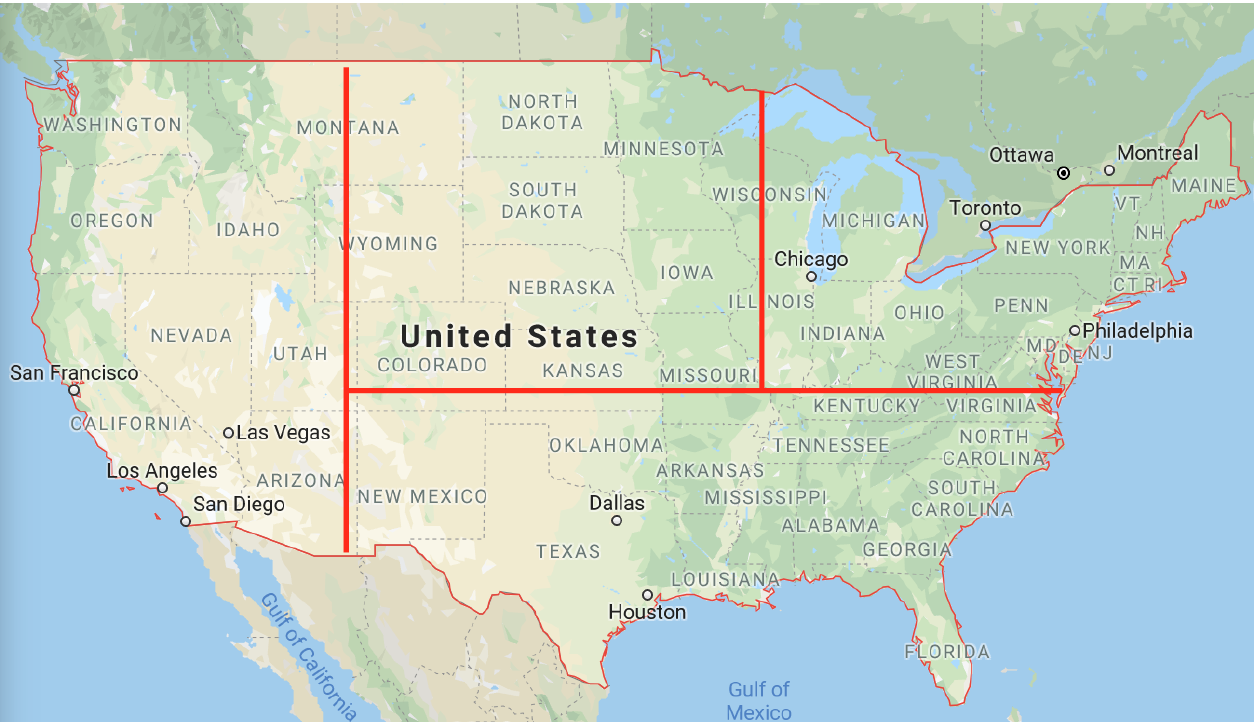
\includegraphics[width = 60mm]{mapDivision}
\end{center}

\bibliographystyle{alpha}
\bibliography{MESgenCov}

\end{document}


